\documentclass[a4paper,kulak]{kulakarticle}

\usepackage[utf8]{inputenc}
\usepackage[dutch]{babel}
\usepackage{listings}
\usepackage{graphicx}
\usepackage{color} %red, green, blue, yellow, cyan, magenta, black, white
\definecolor{mygreen}{RGB}{28,172,0} % color values Red, Green, Blue
\definecolor{mylilas}{RGB}{170,55,241}









\lstset{language=Matlab,%
	%basicstyle=\color{red},
	breaklines=true,%
	morekeywords={matlab2tikz},
	keywordstyle=\color{blue},%
	morekeywords=[2]{1}, keywordstyle=[2]{\color{black}},
	identifierstyle=\color{black},%
	stringstyle=\color{mylilas},
	commentstyle=\color{mygreen},%
	showstringspaces=false,%without this there will be a symbol in the places where there is a space
	numbers=left,%
	numberstyle={\tiny \color{black}},% size of the numbers
	numbersep=9pt, % this defines how far the numbers are from the text
	emph=[1]{for,end,break},emphstyle=[1]\color{red}, %some words to emphasise
	%emph=[2]{word1,word2}, emphstyle=[2]{style},    
}




\date{Academiejaar 2017-2018}
\address{
  Informatica \\
  Numerieke wiskunde \\
  
  Prof. Koen Van Den Abeele
\\
Andries Vansweevelt
}
\title{Verslag project numerieke wiskunde}
\author{Thomas Bamelis en Michiel Provoost}

\begin{document}

\maketitle

\section*{Inleiding}

Dit verslag behandeld de vragen en antwoorden gesteld in het eind-project numerieke wiskunde 2017. De hoofdvraag in dit project is hoe wortels/nulpunten van een willekeurige veelterm kunnen gevonden worden met de methode van Newton-Raphson en de methode van Bairstow. Verder behandelt dit verslag de performantie en fouten op beide algoritmen en  sluit af met deze met elkaar te vergelijken. Beide methoden werden geïmplementeerd in matlab en getest op 10 gegeven veeltermen, met complexe en reële nulpunten. 
Verder werden verschillende opgedragen ease-of-use features geïmplementeerd, zoals een figuur plotten indien enkel de coëfficiënten gegeven.\\
Ook word kort aandacht besteed aan een analyse van een bepaald geval, waarin bekeken wordt welke startwaarden voor beide methoden tot welke (of geen) nulpunten leiden.

\section{Newton-Raphson}
Dit hoofdstuk bespreekt de implementatie van Newton-Raphson, waarin onder andere de methode van Horner, samen met een analyse van de performantie en fouten.

\subsection{Evaluatie veelterm en zijn afgeleide m.b.v. het Hornerschema}
Hier wordt opdracht 1 besproken. \label{sec:horUit} \\~\\
Met het uitgebreide Hornerschema, besproken in \cite{bultheel2006inleiding}, kan een veelterm geëvalueerd in een gegeven punt. Daarna kan met een deel van de oplossing verder gewerkt worden om 1-per-1 de afgeleiden van de veelterm te evalueren in hetzelfde punt.\\

\subsubsection{Implementatie}

Dit werd als volgt geïmplementeerd:\\

\lstinputlisting{../matlab/my_polyval.m}

~\\~\\~\\
Zoals in \cite{bultheel2006inleiding} wordt aangetoond, worden de m eerste afgeleid ( inclusief $f^{(0)}$) gevonden, door m keer het schema van Horner toe te passen op p waarna de functiewaarde van i'de afgeleide gegeven wordt door $k!b^{k+1}_{n-k}$. Merk op dat in de `afgeleide' iteratie, de `afgeleide' - 1 'ste afgeleide behandeld wordt om beter matlabs vector nummering in te kunnen spelen.\\
Het 1'ste element van p, dus de coefficient van de hoogste graad term, wordt nooit aangepast omdat volgens Horner $a_0 = b_0$. Daarna worden de rest van de coefficienten aangepast volgens $b_i = a_i + b_{i-1}*x$. Er wordt rekening gehouden met het feit dat de graad van de veelterm bij iedere iteratie van de afgeleide met 1 verlaagd wordt.
~\\~\\Een bijkomende opdracht was om zo weinig mogelijk geheugen te gebruiken. Om hier mee om te gaan werd in de vector p zelf gewerkt. Dit is geen enkel probleem omdat je nooit de oude vorige elementen nodig hebt en omdat matlab call-by-value is. Dit wil zeggen dat matlab p kopieert en de kopie meegeeft aan de functie waar mee gewerkt mag worden zonder dat de originele p wordt aangepast. 
Het enige geheugen dat extra wordt aangemaakt, is het geheugen gebruikt om de functie waarden terug te geven een de oproeper van de functie.
Dit wil zeggen dat het geheugengebruik van de functie van orde $\Theta( n + m )$ is, met n de graad + 1 van p en m het aantal keer dat afgeleid moet worden.

\subsubsection{Fouten}

De stabiliteit van deze methode komt op 2 manieren in gedrang:
\begin{itemize}
	\item In lijn 45, als p(coefficient) en p(coefficient - 1)*x bijna even groot zijn en tegengesteld teken hebben.
	\item In lijn 52, als de `afgeleide' afgeleide zeer groot word, zullen afrondingsfouten groter worden door de faculteit.
\end{itemize}


\subsection{Een nulpunt vinden met Newton-Raphson}
Hier wordt opdracht 2 besproken.
\\~\\
Indien een willekeurig veelterm gegeven wordt en een startwaarde, kan via de formule van Newton-Raphson (
$x_{i+1} = x_i + \frac{ p(x_i) }{ p^{'}(x_i) }$) een nieuwe x gevonden worden, die dichter bij het nulpunt ligt als er convergentie optreedt.

\subsubsection{Implementatie}
\label{sec:NR}
\lstinputlisting{../matlab/newtonraphson.m}
~\\~\\
Het iteratief berekenen van de volgende x, wordt gestopt op 2 manieren:
\begin{enumerate}
	\item Door de `zwakke' stopwaarde, als de nieuwe x en de vorige x in absolute waarde kleiner zijn dan de meegegeven tolerantie.\\
	In dit geval wordt de functie aanroep als succesvol gezien.
	\item Na 10000 iteraties wordt de lus verplicht afgebroken, om niet in een oneindige lus terecht te komen.
\end{enumerate}

Bij iedere iteratie wordt de `zwakke' fout opnieuw berekent en gecheckt of aan de voorwaarde voldaan wordt.
Op het einde van het algoritme wordt nog een laatste check gedaan om te zien of er voldaan is aan de meegegeven tolerantie. Indien wel wordt de gevonden benadering van het nulpunt meegegeven, anders NaN.
Er werd nog een extra geïmplementeerd om de stabiliteit te bevorderen die in de volgende sectie besproken wordt.

\subsubsection{Fouten}
De grootste fout wordt verkregen door een kleine $p^{'}(x_i)$ in de berekening van een nieuwe x, door de deling in lijn 77. Om hiermee om te gaan wordt indien $p^{'}(x_i)$ kleiner dan 1 wordt, in de deling een $p^{'}(x_i)$ vermenigvuldigt wordt met 100 om het verderzetten van de fout op $p^{'}(x_i)$ te verzachten. Hierna wordt de volledige quotiënt opnieuw vermenigvuldigt met 100. De 100 kan groter genomen worden, maar dan worden de afrondingsfouten voor een grote $p(x)_i$ ook groter.

\subsection{Deflatie met Horner}
Hier wordt opdracht 3 besproken.\\~\\
Nadat een nulpunt met Newton-Raphson gevonden wordt, kan de (x - gevondenNulpunt) factor weggedeeld worden met het alom bekende schema van Horner. 
Er moest ook voorzien worden dat als het gegeven nulpunt complex is, zijn complex toegevoegde ook weggedeeld wordt.
\subsubsection{Implementatie}
\lstinputlisting{../matlab/horner.m}
~\\~\\
De implementatie is gelijk aan die van sectie \ref{sec:horUit} met 1 iteratie, waarbij de eerste n-1 coëfficiënten worden teruggegeven na de iteratie. Dit stelt dus een veelterm van 1 graad lager dan p voor. Dit geld echter enkel als het nulpunt reëel is. 
In dit geval word een veelterm die 2 graden lager is dan p teruggegeven, waaruit beide nulpunten op dezelfde manier zijn weggedeeld. Tijdens het wegdelen van het complex toegevoegde wordt dus met een input van 1 graad lager een output van 2 graden lager gegeven.

\subsubsection{Fouten}

De stabiliteit van deze methode lijd onder dezelfde problemen als \ref{sec:horUit}:
\begin{itemize}
	\item In lijn 50, als p(coefficient) en q(coefficient - 1)*x bijna even groot zijn en tegengesteld teken hebben.
	\item In lijn 77, als a(coefficient) en q(coefficient - 1)*x bijna even groot zijn en tegengesteld teken hebben.
\end{itemize}

\subsection{Alle nulpunten vinden}
Hier wordt opdracht 3 besproken.\\~\\
Met de hiervoor besproken methoden werd zoals gevraagd een implementatie geschreven die alle nulpunten berekent van een gegeven veelterm. Deze methode vraagt om een veelterm, een startwaarde en een tolerantie die $10^{-6}$ is indien niet meegegeven. Er wordt een nulpunt bepaald met de methode van Newton-Raphson met de gegeven startwaarde, waarna dit nulpunt weggedeeld wordt met de methode van Horner. Er wordt met de nieuwe veelterm die door Horner werd teruggegeven verder gewerkt en er wordt opnieuw een nulpunt met Newton-Raphson bepaald met als startwaarde het vorige gevonden nulpunt.
\\
Dit wordt gedaan tot alle nulpunten van de veelterm gevonden worden.
\\
Als Newton-Raphson niet convergeert, en dus NaN wordt teruggegeven, wordt de huidige functie geplot en om een nieuw startpunt gevraagd aan de gebruiker.\\
Uiteindelijk wordt een vector met alle nulpunten van p teruggegeven.

\subsubsection{Implementatie}
\lstinputlisting{../matlab/newtonraphsondef.m}
~\\~\\

\subsubsection{Fouten}
Omdat deze functie op zich niet veel rekenwerk bevat, maar dit wordt doorgegeven aan de opgeroepen functie, kan hier niet veel over de fout gepraat worden.
\\
Bij het plotten van de functie zijn kleine fouten niet zo belangrijk, omdat dit op een grote schaal gebeurt en omdat een plot sowieso nooit als betrouwbaar mag gezien worden.

\section{Bairstow}
De methode van Bairstow werkt door telkens bij iedere stap 2 nulpunten af te zonderen. Dit zorgt ervoor dat de methode nog sneller convergeert. Wel hebben we om dit efficiënt te doen verlopen het dubbelrijige Hornerschema nodig. Dit hoofdstuk bespreekt de implementatie van dat schema, de implementatie van het algoritme van Bairstow zelf en hoe we dan een algoritme implementeren die aan de hand van de methode van Bairstow alle nulpunten van een gegeven veelterm teruggeeft.

\subsection{Evaluatie via dubbelrijige Horner}

Om de 2 nulpunten effeciënt te kunnen evalueren is er een nieuwe functie geïmplementeerd die het dubbelrijige algoritme van Horner gebruikt. Dit laat ons toen om in $(2n+1)V$ en $2nO$ de beide te evalueren in plaats van $(4n-2)V$ en $(3n-2)O$ \cite{bultheel2006inleiding}.

\subsubsection{Implementatie}
\lstinputlisting{../matlab/doubleHorner.m}
~\\~\\
De implementatie heeft invloeden met die van sectie \ref{sec:horUit} met 1 iteratie. Echter zal nu bij elke coëfficiënt direct het gevolg van het afzonderen van beide nulpunten in rekening worden gebracht. Daarom baseert deze methode zich ook op de 2 voorgaande coëfficiënten. wat de basisstap wat uitgebreider maakt. De methode berekent dus een veelterm van 2 graden lager dan p. 

\subsubsection{Fouten}

De stabiliteit van deze methode lijd onder dezelfde problemen als \ref{sec:horUit}:
\begin{itemize}
	\item In lijn 28, als p(2) en q(1)*rho bijna even groot zijn en tegengesteld teken hebben.
	\item In lijn 34, als p(graad) en q(graad - 1)*rho of q(graad - 1)*rho en -q(graad-2)*mu bijna even groot zijn en tegengesteld teken hebben.
\end{itemize}
\subsubsection{Vinden van de 2 nulpunten uit de 2de-graadsfunctie}
Hier wordt opdracht 5 besproken.
\\~\\
Omdat Bairstow telkens een 2-de graadsveelterm afzondert, hebben we nog een methode nodig die efficiënt de wortels uit die veelterm haalt. Daarvoor gebruiken we de functie quadroots. Deze berekent de 1 wortel uit de veelterm en gaat dan iteratief tewerk om de 2e wortel te bepalen.

\subsubsection{Implementatie}
\lstinputlisting{../matlab/quadroots.m}
~\\~\\

Een nuttige extra parameter en bijdrage aan de implementatie zou zijn dat men kan de stabiliteitsverhoger instellen naargelang de grootte van het probleem. Dit zou de robuustheid van het algoritme zeker ten goede komen.

\subsection{Een nulpunt vinden met Bairstow}
Hier wordt opdracht 6 besproken.
\\~\\
Indien een willekeurig veelterm gegeven wordt en 2 startwaardes, kan via de formules van Bairstow een nieuwe $\rho$ en $\mu$ gevonden worden, die dichter bij het nulpunt ligt als er convergentie optreedt. Doordat we telkens 2 nulpunten afzonderen zal deze kwadratisch convergeren.

\subsubsection{Implementatie}

\lstinputlisting{../matlab/bairstow.m}

~\\~\\
Het iteratief berekenen van de volgende $\rho$ en $\mu$, wordt op eenzelfde manier gestopt als \ref{sec:NR}.

\subsubsection{Fouten}
De grootste fout wordt verkregen door een kleine D in de berekening van $\delta \rho$ en $\delta \mu$, door de deling in lijn 85 en 86.

\subsection{Alle nulpunten vinden}
Hier wordt opdracht 7 besproken.
\\~\\
Met al deze werd zoals gevraagd een implementatie gemaakt die alle nulpunten berekent van een gegeven veelterm. Deze methode vraagt om een veelterm, 2 (mogelijks complexe) startwaarden en een tolerantie die $10^{-6}$ is indien niet meegegeven. Er worden 2 nulpunten bepaald met de methode van Bairstow met de gegeven startwaarde, waarna die nulpunten weggedeeld wordt met de methode van de dubbelrijige Horner. Er wordt met de nieuwe veelterm die door Horner werd teruggegeven verder gewerkt en er wordt opnieuw een nulpunt met Bairstow bepaald met als startwaarden de vorige gevonden nulpunten. Indien de graad van p nu kleiner zou zijn dan 2, dan kunnen we rechtstreeks het laatste nulpunt berekenen.
\\
Dit wordt gedaan tot alle nulpunten van de veelterm gevonden worden.
\\
Als Bairstow niet convergeert, en dus NaN wordt teruggegeven, wordt de huidige functie geplot en om  nieuwe startpunten gevraagd aan de gebruiker.\\
Uiteindelijk wordt een vector met alle nulpunten van p teruggegeven.

\subsubsection{Implementatie}
\lstinputlisting{../matlab/bairstowdef.m}
~\\~\\

\subsubsection{Fouten}
Deze functie zelf bevat opnieuw niet veel pijnpunten. 
\\
Het plotten voldoet aan dezelfde voorwaarden als bij Newton-Raphson.

\section{testen van robuustheid}
Hier wordt opdracht 8 besproken.
\\~\\
Beide functies (newtonraphsondef en bairstowdef) werden uitgevoerd op de volledige testbank. Daaruit bleek dat Newton-Raphson minder snel gaat convergeren dan Bairstow. Maar beide implementaties leverden betrouwbare resultaten en kunnen toch als robuust beschouwd worden.

\section{Convplot}
Hier wordt opdracht 9 besproken.
\\~\\
Er zijn verschillende implementaties voor convplot, en deze worden apart besproken.
\subsection{convplot voor Newton-Raphson}
De convplot voor Newton-Raphson is als volgt geïmplementeerd:
\lstinputlisting{../matlab/convplotnr.m}
~\\~\\
Wat we in feite doen is een lijst opstellen met voor elke nulwaarde van newtonraphsondef op onze gegeven starwaarde een kleur. En dan de gehele lijst met mogelijke startwaarden overlopen en dan kijken welk punt (binnen de tolerantie) gelijk is aan het verkregen nulpunt. Indien we een Nan terugkregen plotten we een rood punt.
\subsection{convplot voor Bairstow}
De convplot voor Bairstow is als volgt geïmplementeerd:
\lstinputlisting{../matlab/convplotbr.m}
~\\~\\
Deze implementatie is in feite bijna identiek aan die van Newton-Raphson. Behalve dat we moeten rekening houden met het feit dat we 2 nulpunten kunnen meekrijgen.

\subsection{convplots van Bairstow en Newton-Raphson}
Hier wordt opdracht 10 besproken.
\\~\\
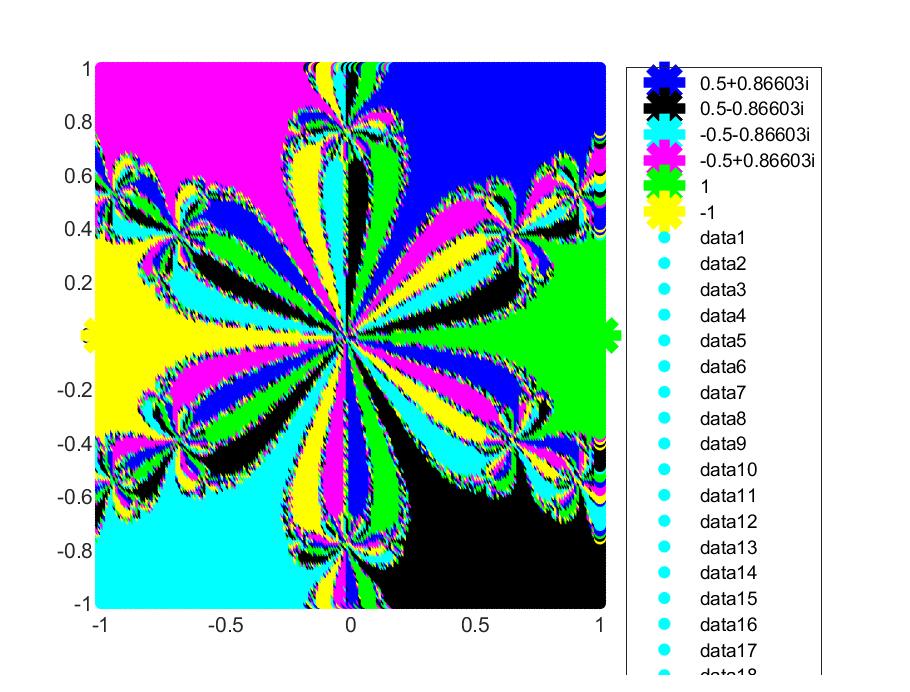
\includegraphics[]{nrPlot}
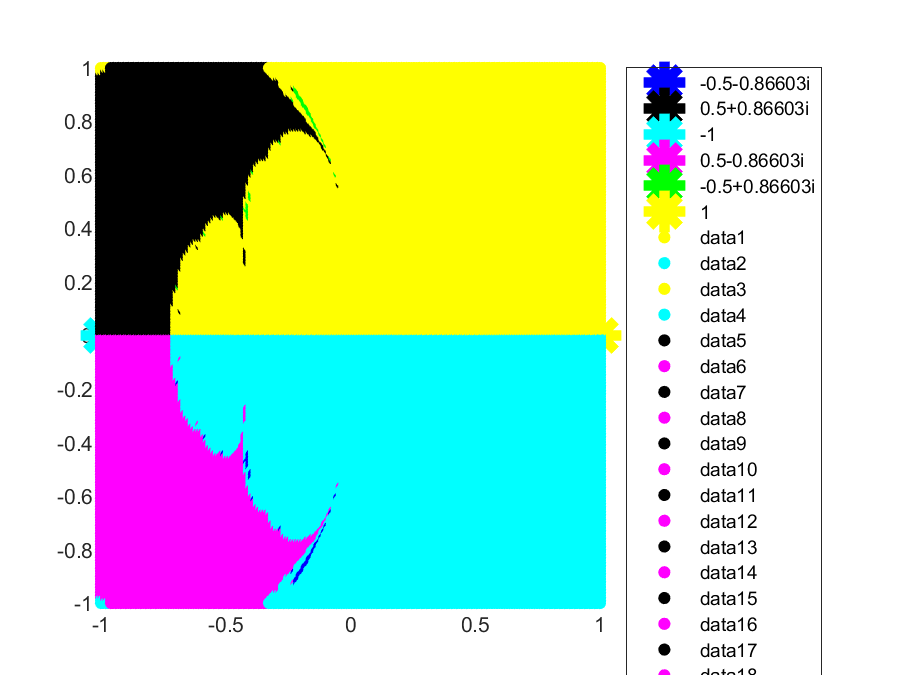
\includegraphics[]{brPlot}
We kunnen enkel dingen toch duidelijk aanhalen uit de 2 plots:
\begin{itemize}
	\item Bairstow heeft veel minder logische en gelijk verdeelde vlakken. Dit komt waarschijnlijk door de grote sprongen die het kan maken. Dit omdat het met 2 variabelen werkt.
	\item Newton-Raphson heeft een zeer afgebakende structuur en alles convergeert naar iets in de dichte omgeving. Dit waarschijnlijk omdat de afgeleiden ervoor zorgen dat we aan een soort van hillclimbing gaan doen.
	\item Aan de randen van Bairstow kunnen we waar nemen dat we convergeren naar totaal andere punten. Deze zone is zeer klein in vergelijking met de geweven structuur van Newton-Raphson. We kunnen dus veel beter voorspellen waarnaar een punt zal convergeren bij Bairstow als we de algemene plot weten. Terwijl Newton-Raphson duidelijker rond het punt convergeert maar minder voorspelbaar is op de randen.
\end{itemize}


\section{Newton-Raphson VS Bairstow}
Hier wordt opdracht 11 besproken.
\\~\\
Men kan zien dat Bairstow heel wat complexer is dan Newton-Raphson en ook altijd convergeert. Het convergeert ook in veel groter zones dan Newton-Raphson. Bairstow laat wel veel meer ruimte voor het opblazen van fouten en is een stuk geheugenintensiever dan newton-Raphson. Men kan zelf op beperkte instanties op beperkte machines een verschil in performatie voelen. Maar het geeft wel over het algemeen de beste resultaten en convergeert dus ook veel sneller. Het zal dus een betere methode zijn, maar om op krachtigere machines te draaien.

\section*{Besluit}

We zien dat Newton-Raphson en bairstow vrij eenvoudige theoretische modellen zijn, maar dat deze we vrij snel door kleine verschillen zich van elkaar onderscheiden. De implementatie is ook een stuk verschillend. Toch komen de pijnpunten in vorm grotendeels overeen.


\bibliographystyle{unsrt}
\bibliography{verslag}

\end{document}
